\chapter{Results}
\label{ch:results}

\section{Reproduction and Verification of Results}
\label{ch:results-reproduction}

Given that this thesis draws heavily upon the research conducted by \cite{kotelnikov2022TabDDPMModellingTabular},
it was deemed absolutely necessary to first reproduce the original experiments and subsequently verify the authors findings,
prior to conducting any new experiments.
Fortunately, the publicly available code \cite{akim2023TabDDPMModellingTabular}, facilitated the replication of the experiments with relative ease.

The reproduction is limited to the adult dataset from \autoref{ch:methods-datasets} and to the machine learning efficacy computed with regards to a tuned CatBoost \cite{prokhorenkova2018CatBoostUnbiasedBoosting} model.

Firstly, a CatBoost model was tuned on the adult dataset, using the provided tuning script (tune\_evaluation\_model.py) [TODO: Drin lassen oder weg lassen?].
Next, for each sampling algorithm, a model was trained, according to the configuration files provided by the authors.
Each configuration file contains the parameters the authors found during hyperparameter tuning.
Hence, with the models respective pipeline.py script, the best found model from hyperparameter tuning could be trained and saved.
Finally, the trained CatBoost and trained sampling model were used in the evaluation script (eval\_seeds.py), which calculates and reports the results.

\begin{table}[h]
	\centering
	\begin{tabular}{l|c|c|r}
		\hline
		\textbf{Model}     & \textbf{Reproduction} & \textbf{Original} & \textbf{Difference} \\ \hline
		Real               & 0.815                 & 0.815             & 0                   \\ \hline
		TVAE$^{ml}$        & 0.780                 & 0.781             & -0.001              \\ \hline
		CTABGAN$^{ml}$     & 0.775                 & 0.783             & -0.008              \\ \hline
		CTABGAN+$^{ml}$    & 0.775                 & 0.772             & +0.003              \\ \hline
		SMOTE$^{ml}$       & 0.791                 & 0.791             & 0                   \\ \hline
		TabDDPM$^{ml}_{q}$ & 0.794                 & 0.795             & -0.001              \\ \hline
	\end{tabular}
	\caption[Reproduction of original Results]{Comparison of the CatBoost F1-score on synthetic datasets, created by different sampling models.
		F1-Scores of the reproduction experiments are compared against the results reported by the original authors \cite[Table 4, p. 8]{kotelnikov2022TabDDPMModellingTabular}.}
	\label{tab:reproduction}
\end{table}

\autoref{tab:reproduction} shows the computed F1-scores achieved by the CatBoost model when trained on different synthetic datasets generated by different sampling models.
The scores that could be reproduced are almost exactly the same as the scores reported by the original authors.
All differences are within the standard deviation reported by the authors, except for the CTABGAN-model.
It is unclear, why the CTABGAN-model score deviates in the reproduction experiment from the original score.
It is important to note, that minor modifications to the code or different python library versions have caused this alternation, which where required in order to train the model in the cloud environment, specified in \autoref{ch:methods-experimentalSetup}.

Therefore, the results as reported by the authors could be overall reproduced and verified.

\section{Metric Results}
\label{ch:results-Metric-results}

% QUALITATIVE vs QUANTITIVE

\subsection{Baseline Experiments}
\label{ch:Baseline}

After verification that the models are able to reproduce the machine-learning efficacy scores as reported,
their performance is additionally evaluated using the similarity evaluation as proposed in \autoref{ch:conceptualDesign-Evaluation}.
\autoref{tab:ml_baseline} shows the complete machine learning efficacy score results for the different sampling techniques:

\begin{table}[h]
	\centering
	\begin{tabular}{l|c|c|c}
		\hline
		\textbf{Model}     & \textbf{Accurarcy} & \textbf{F1}    & \textbf{ROC-AUC} \\ \hline
		Real               & 0.874              & 0.815          & 0.928            \\ \hline
		TVAE$^{ml}$        & 0.845              & 0.781          & 0.900            \\ \hline
		CTABGAN$^{ml}$     & 0.850              & 0.775          & 0.900            \\ \hline
		CTABGAN+$^{ml}$    & 0.855              & 0.775          & 0.907            \\ \hline
		SMOTE$^{ml}$       & 0.858              & 0.791          & 0.910            \\ \hline
		TabDDPM$^{ml}_{q}$ & \textbf{0.860}     & \textbf{0.794} & \textbf{0.913}   \\ \hline
	\end{tabular}
	\caption[Machine learning efficacy baseline]{Machine learning efficacy (CatBoost) baseline results.}
	\label{tab:ml_baseline}
\end{table}


In addition to the machine learning efficacy scores, the similarity scores of the TabSynDex metric are computed (\autoref{tab:sim_baseline}).

\begin{table}[h]
	\centering
	\begin{tabular}{lrrrrrr}
		\toprule
		\textbf{Model}     & \textbf{Similarity Score} & \textbf{Basic} & \textbf{Correlation} & \textbf{ML}    & \textbf{Support} & \textbf{pMSE}  \\
		\midrule
		Real               & 0.960                     & 0.992          & 0.943                & 0.998          & 0.984            & 0.882          \\
		TVAE$^{ml}$        & 0.658                     & 0.854          & 0.814                & 0.962          & 0.657            & 0.000          \\
		CTABGAN$^{ml}$     & 0.741                     & 0.940          & 0.832                & 0.984          & \textbf{0.947}   & 0.000          \\
		CTABGAN+$^{ml}$    & 0.750                     & 0.969          & 0.882                & 0.990          & 0.892            & 0.019          \\
		SMOTE$^{ml}$       & 0.723                     & 0.953          & 0.865                & \textbf{0.992} & 0.804            & 0.000          \\
		TabDDPM$^{ml}_{q}$ & \textbf{0.759}            & \textbf{0.973} & \textbf{0.919}       & \textbf{0.992} & 0.874            & \textbf{0.035} \\
		\bottomrule
	\end{tabular}
	\caption[Similarity baseline]{Similarity baseline results using the TabSynDex metrices. Similarity Score is the average of the other five scores. Best result is highlighted in bold}
	\label{tab:sim_baseline}
\end{table}

These baseline experiments show, that the Diffusion based synthesis approach outperforms other models not only in terms of machine learning efficacy, but also in terms of other metrics.
However, \autoref{tab:sim_baseline} shows that the CTABGAN models outperform TabDDPM in the Support coverage metric.
Additionally, it is worth mentioning that even though TabDDPM achieves the highest \gls{pmse} score, it is still extremely low and almost 0, which is the same for all other models.
The authors of \cite{chundawat2022UniversalMetricRobust} essentially confirm this observation.
During their experiments, the tested sampling techniques (various \gls{gan}-based approaches) also struggle to produce any synthetic data which achieves a \gls{pmse} score that is noticeably higher than 0.
\autoref{tab:sim_baseline} indicates, that this observation also holds for a diffusion based approach, which hyperparameters were tuned towards a machine learning efficacy score using a CatBoost model.

\subsection{Experiment 1: Adding Tabular Processing}
\label{ch:Experiment-1}

In the first set of experiments, the different tabular processing mechanism described in \autoref{ch:architecture-tabularProcessor-implementations} are evaluated.
For this, the tabular processing mechanisms have been added to the pipeline of TabDDPM, as described in the concept in \autoref{fig:Overall_changed}.
Consequently, the tuning (tune\_ddpm.py, see \autoref{ch:scripts}) of the diffusion model with the additional tabular processing was required.
The models hyperparameter have again been tuned towards the machine learning efficacy of a CatBoost model.

The results of the machine learning efficacy and TabSynDex metric results can be found in \autoref{tab:exp1-ml} and \autoref{tab:exp1-sim} respectively.
\begin{table}[h]
	\centering
	\begin{tabular}{lrrr}
		\toprule
		\textbf{Model}         & \textbf{Accurarcy} & \textbf{F1}    & \textbf{ROC-AUC} \\
		\midrule
		Real                   & 0.874              & 0.815          & 0.928            \\
		TabDDPM$^{ml}_{q}$     & 0.860              & 0.794          & 0.913            \\
		TabDDPM-BGM$^{ml}_{q}$ & \textbf{0.863}     & \textbf{0.798} & \textbf{0.916}   \\
		TabDDPM-FT$^{ml}_{q}$  & 0.785              & 0.552          & 0.821            \\
		\bottomrule
	\end{tabular}
	\caption[Experiment1-ML-Efficacy]{CatBoost Machine learning efficacy scores for different tabular processing techniques.}
	\label{tab:exp1-ml}
\end{table}

\begin{table}[h]
	\centering
	\begin{tabular}{lrrrrrr}
		\toprule
		\textbf{Model}         & \textbf{Similarity Score} & \textbf{Basic} & \textbf{Correlation} & \textbf{ML}    & \textbf{Support} & \textbf{pMSE}  \\
		\midrule
		Real                   & 0.960                     & 0.992          & 0.943                & 0.998          & 0.984            & 0.882          \\
		TabDDPM$^{ml}_{q}$     & \textbf{0.759}            & \textbf{0.973} & \textbf{0.919}       & 0.992          & 0.874            & \textbf{0.035} \\
		TabDDPM-BGM$^{ml}_{q}$ & 0.742                     & 0.964          & 0.918                & \textbf{0.996} & 0.831            & 0.000          \\
		TabDDPM-FT$^{ml}_{q}$  & 0.595                     & 0.495          & 0.648                & 0.869          & \textbf{0.963}   & 0.000          \\
		\bottomrule
	\end{tabular}
	\caption[Experiment1-Similarity]{TabSynDex evaluation metric scores for different tabular processing techniques.}
	\label{tab:exp1-sim}
\end{table}

Both evaluations show, that the additional \gls{bgm} tabular processing seems to increase the ML-efficacy scores.
All metrics in \autoref{tab:exp1-ml} are highest for the TabDDPM-BGM model and the ML efficacy score of TabSynDex (which makes use of different models)
is highest for TabDDPM-BGM as well, although only by a slight margin.
\autoref{tab:exp1-sim} indicates, that this increase seems to come at the cost of reduced performance in the other metrices, which are highest for the Basic-, Correlation- and pMSE-Score for the plain TabDDPM version.
TabDDPM-FT compares significantly worse than its counterparts in the Correlation and Basic similarity score.
Interestingly, TabDDPM-FT performance significantly better in the Support score than the other versions and approximately 13 percentage-points worse in terms of ML efficacy computed by the TabSynDex metric.
More details can be seen in the \autoref{tab:exp1-ml}, that shows that especially the F1 score from TabDDPM-FT is much worse than the F1 score of the other models.
Lastly, neither the \gls{bgm} nor the \gls{ft} tabular processing enable the diffusion model to produce synthetic data that is able to increase the \gls{pmse} score.


\subsection{Experiment 2: Similarity Hyperparameter optimization}
\label{ch:Experiment-2}

The second set of experiments are very similar to the first experiments.
Instead of tuning the models hyperparameters after the machine learning efficacy, as proposed by the original authors,
the models hyperparameters are tuned after the TabSynDex similarity score.

The results of the machine learning efficacy and TabSynDex metric results can be found in \autoref{tab:exp2-ml} and \autoref{tab:exp2-sim} respectively.

TODO FT simTune; ctabgan+simTUne

\begin{table}[h]
	\centering
	\begin{tabular}{lrrr}
		\toprule
		\textbf{Model}        & \textbf{Accurarcy} & \textbf{F1}    & \textbf{ROC-AUC} \\
		\midrule
		Real                  & 0.874              & 0.815          & 0.928            \\
		TabDDPM$^{s}_{q}$     & 0.856              & 0.782          & 0.908            \\
		TabDDPM-BGM$^{s}_{q}$ & \textbf{0.859}     & \textbf{0.792} & \textbf{0.911}   \\
		TabDDPM-FT$^{s}_{q}$  & 0.767              & 0.450          & 0.712            \\
		CTABGAN$^{s}$         & 0.850              & 0.776          & 0.900            \\
		TVAE$^{s}$            & 0.845              & 0.780          & 0.900            \\
		\bottomrule
	\end{tabular}
	\caption[Experiment2-ML-Efficacy]{CatBoost Machine learning efficacy scores for different tabular processing techniques which hyperparameter have been tuned towards the TabSynDex similarity score.}
	\label{tab:exp2-ml}
\end{table}

\begin{table}[h]
	\centering
	\begin{tabular}{lrrrrrr}
		\toprule
		\textbf{Model}        & \textbf{Similarity Score} & \textbf{Basic} & \textbf{Correlation} & \textbf{ML}    & \textbf{Support} & \textbf{pMSE}  \\
		\midrule
		Real                  & 0.960                     & 0.992          & 0.943                & 0.998          & 0.984            & 0.882          \\
		TabDDPM$^{s}_{q}$     & 0.852                     & 0.976          & \textbf{0.921}       & \textbf{0.991} & 0.952            & 0.420          \\
		TabDDPM-BGM$^{s}_{q}$ & \textbf{0.857}            & \textbf{0.982} & 0.858                & \textbf{0.991} & 0.920            & \textbf{0.532} \\
		TabDDPM-FT$^{s}_{q}$  & 0.589                     & 0.513          & 0.620                & 0.819          & \textbf{0.992}   & 0.000          \\
		CTABGAN$^{s}$         & 0.740                     & 0.938          & 0.833                & 0.984          & 0.947            & 0.000          \\
		TVAE$^{s}$            & 0.658                     & 0.856          & 0.815                & 0.962          & 0.656            & 0.000          \\
		\bottomrule
	\end{tabular}
	\caption[Experiment2-Similarity]{TabSynDex evaluation metric scores for different tabular processing techniques which hyperparameter have been tuned towards the TabSynDex similarity score.}
	\label{tab:exp2-sim}
\end{table}

The results show, that TabDDPM-BGM outperforms all other models in terms of the CatBoost machine learning efficacy and is on pair with TabDDPM in the TabSynDex ML-efficacy score.
TabDDPM-BGM also has the highest overall Similarity Score and achieves the highest Basic score and \gls{pmse} score.
The simpler TabDDPM however outperforms its \gls{bgm} counterpart in terms of Correlation and Support score.
Overall, TabDDPM achieves comparable performance to TabDDPM-BGM on all metrics, with the biggest difference in the \gls{pmse} score of - 11 percentage points.
TabDDPM-FT performance significantly worse than all other TabDDPM variants in all metrics except the support score.
On the one hand, it seems to be the case that hyperparameter tuning after the similarity score does have a big influence on the TabDDPM and TabDDPM-BGM models \gls{pmse} score.
On the other hand, this hyperparameter tuning did not affect the \gls{pmse} score of the other tested model, the CTABGAN, TVAE or the TabDDPM-FT.

\subsection[]{Experiment 3: Exchanging the Normalization}
\label{ch:Experiment-3}

So far, all TabDDPM models received data, that was normalize according to the quantile-transform function (applied after tabular processing), as proposed in \cite{kotelnikov2022TabDDPMModellingTabular}.
In a third experiment, it will be investigated how the models perform, when their quantile-transform function is replaced by a more simple MinMax-scaler, as explained in \autoref{sec:dataNormalization}.
Based upon the performance of the model variants so far, only the plain TabDDPM and TabDDPM-BGM, tuned after the similarity score have been investigated, since the performance of TabDDPM-FT was noticeably worse.


\begin{table}[h]
	\centering
	\begin{tabular}{lrrr}
		\toprule
		\textbf{Model}        & \textbf{Accurarcy} & \textbf{F1}    & \textbf{ROC-AUC} \\
		\midrule
		Real                  & 0.874              & 0.815          & 0.928            \\
		TabDDPM$^{s}_{m}$     & 0.856              & 0.778          & \textbf{0.910}   \\
		TabDDPM-BGM$^{s}_{m}$ & \textbf{0.857}     & \textbf{0.787} & 0.909            \\
		\bottomrule
	\end{tabular}
	\caption[Experiment3-ML-Efficacy]{CatBoost Machine learning efficacy scores for different tabular processing techniques which hyperparameter have been tuned towards the TabSynDex similarity score
		and the data was transformed according to a MinMax-scaler.}
	\label{tab:exp3-ml}
\end{table}

\begin{table}[h]
	\centering
	\begin{tabular}{lrrrrrr}
		\toprule
		\textbf{Model}        & \textbf{Similarity Score} & \textbf{Basic} & \textbf{Correlation} & \textbf{ML}    & \textbf{Support} & \textbf{pMSE}  \\
		\midrule
		Real                  & 0.960                     & 0.992          & 0.943                & 0.998          & 0.984            & 0.882          \\
		TabDDPM$^{s}_{m}$     & \textbf{0.869}            & 0.938          & \textbf{0.930}       & 0.990          & \textbf{0.928}   & \textbf{0.558} \\
		TabDDPM-BGM$^{s}_{m}$ & 0.856                     & \textbf{0.981} & 0.913                & \textbf{0.992} & 0.915            & 0.476          \\
		\bottomrule
	\end{tabular}
	\caption[Experiment3-Similarity]{TabSynDex evaluation metric scores for different tabular processing techniques which hyperparameter have been tuned towards the TabSynDex similarity score
		and the data was transformed according to a MinMax-scaler.}
	\label{tab:exp3-sim}
\end{table}

Given the results in \autoref{tab:exp3-ml} and \autoref{tab:exp3-sim} it seems to be the case that TabDDPM-BGM outperforms TabDDPM in terms of ML-efficacy and the Basic score, but only by a slight margin.
TabDDPM, on the other hand, achieves a higher overall similarity score, mainly due to the superior performance in the Correlation, Support and pMSE-score.


\section{Visual Results}
\label{ch:results-Visual}

Several plots have been produced accroding to the methodology of \cite{brenninkmeijer2019GenerationEvaluationTabular}.
This section will cover which plots have been produced and how the plots for different model versions are different.

\subsection[]{Correlation Difference Matrix}

To get an intuition on how well correlations within the dataset are reproduced, correlation matrices have been computed.
The correlation matrix for the synthetic dataset has been subtracted from the correlation matrix of the real dataset in order to produce a correlation difference matrix.
The smaller the difference, the more similar are the correlations within the synthetic dataset to the correlations within the real dataset.

Looking at the correlations matrix differences in \autoref{fig:corr_base} for the baseline models that are not diffusion based, one can see that the CTABGAN+$^{ml}$ and SMOTE approaches have the smallest
correlation matrix difference.
However, the diffusion model TabDDPM$^{ml}$ produces the matrix with the smallest overall differences.

\begin{figure}[h]
	\centering
	\begin{subfigure}{0.3\textwidth}
		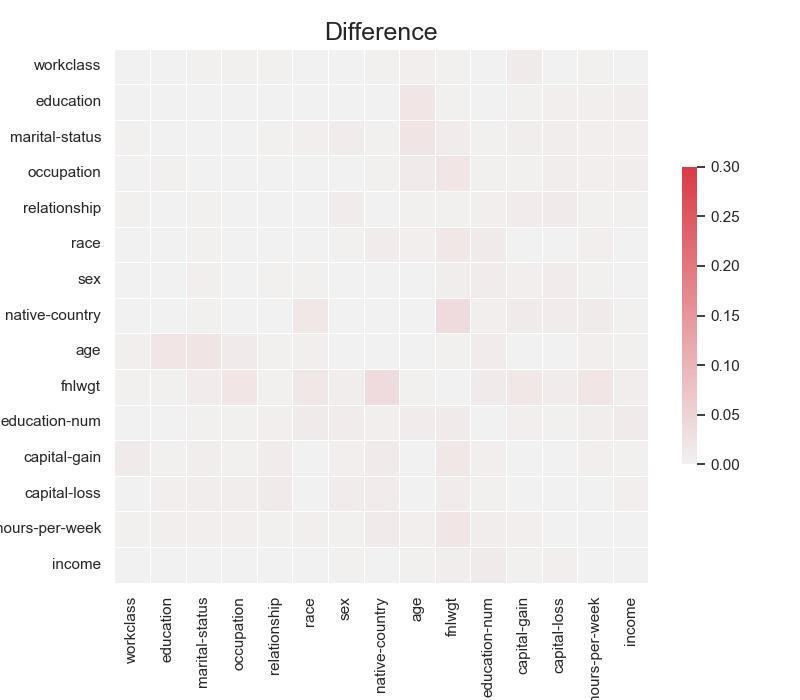
\includegraphics[width=\textwidth]{images/correlation_difference/real.jpg}
		\caption{Real}

	\end{subfigure}
	\hfill
	\begin{subfigure}{0.3\textwidth}
		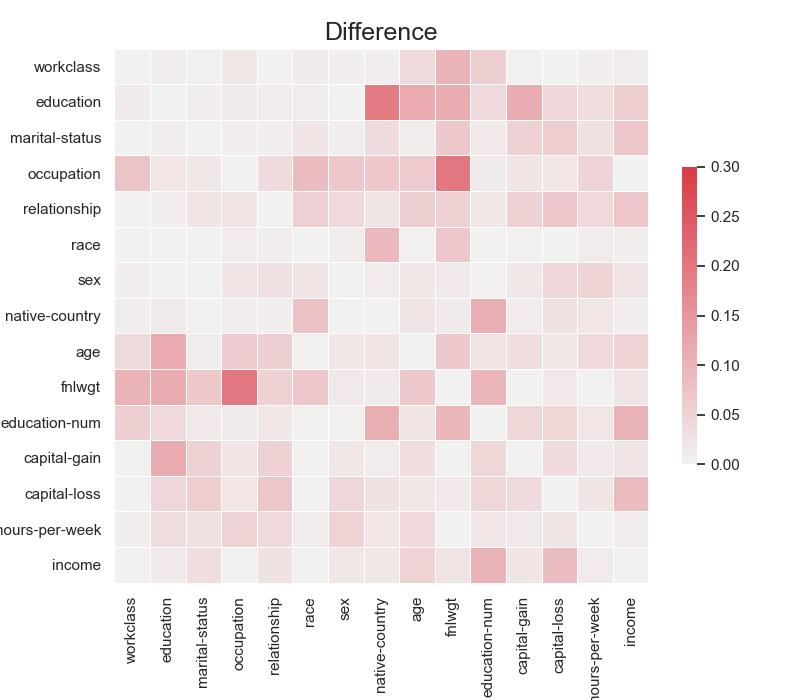
\includegraphics[width=\textwidth]{images/correlation_difference/tvae.jpg}
		\caption{TVAE$^{ml}$}

	\end{subfigure}
	\hfill
	\begin{subfigure}{0.3\textwidth}
		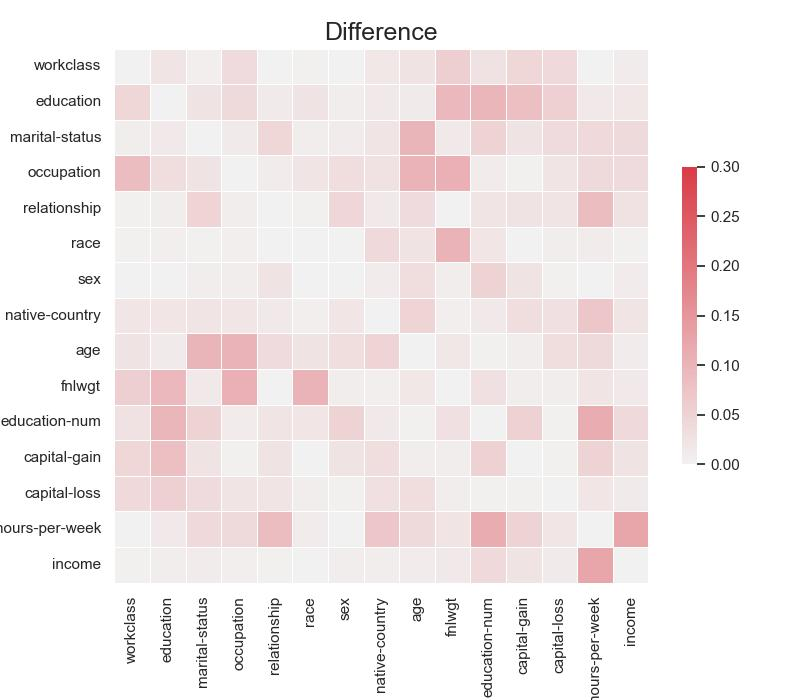
\includegraphics[width=\textwidth]{images/correlation_difference/ctabgan.jpg}
		\caption{CTABGAN$^{ml}$}
	\end{subfigure}

	\begin{subfigure}{0.3\textwidth}
		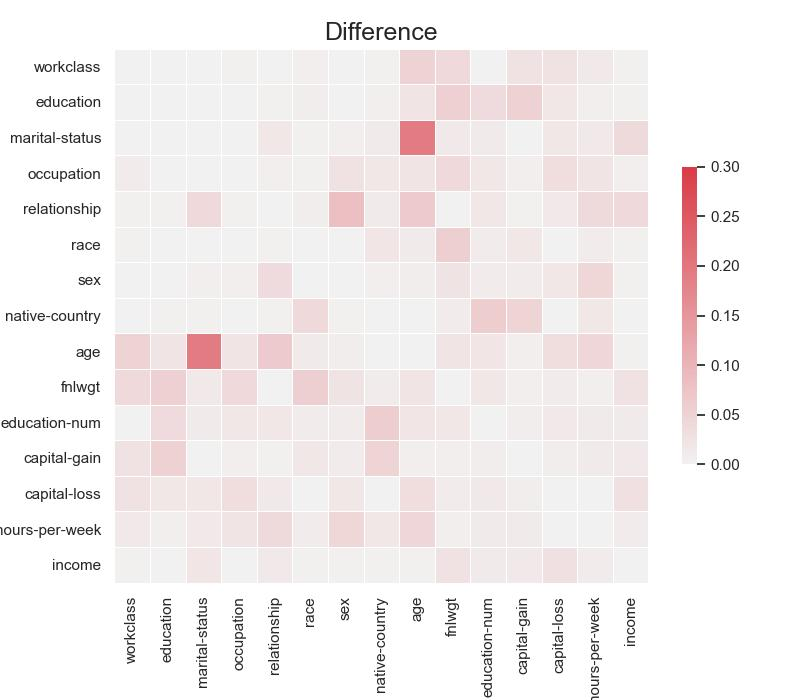
\includegraphics[width=\textwidth]{images/correlation_difference/ctabgan+.jpg}
		\caption{CTABGAN+$^{ml}$}

	\end{subfigure}
	\begin{subfigure}{0.3\textwidth}
		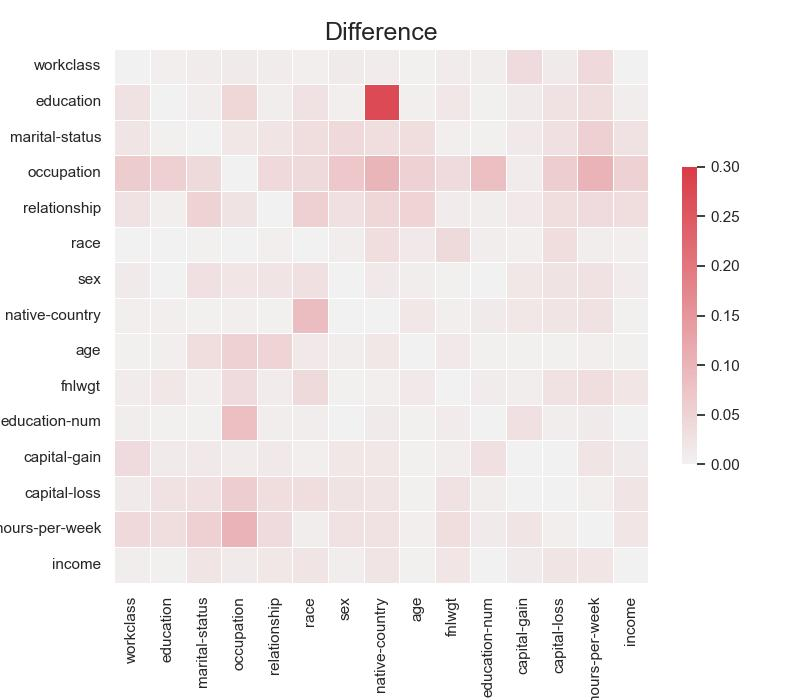
\includegraphics[width=\textwidth]{images/correlation_difference/smote.jpg}
		\caption{SMOTE}

	\end{subfigure}
	\begin{subfigure}{0.3\textwidth}
		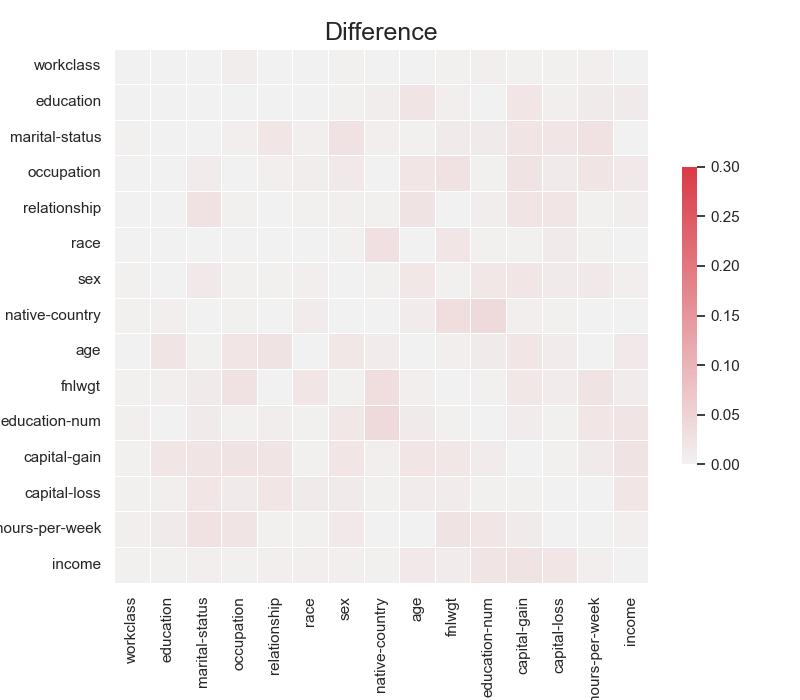
\includegraphics[width=\textwidth]{images/correlation_difference/tab-ddpm.jpg}
		\caption{TabDDPM$^{ml}_q$}

	\end{subfigure}
	\caption{Correlation Matrix difference for Baseline models.}
	\label{fig:corr_base}
\end{figure}


\begin{figure}[h]
	\begin{subfigure}{0.3\textwidth}
		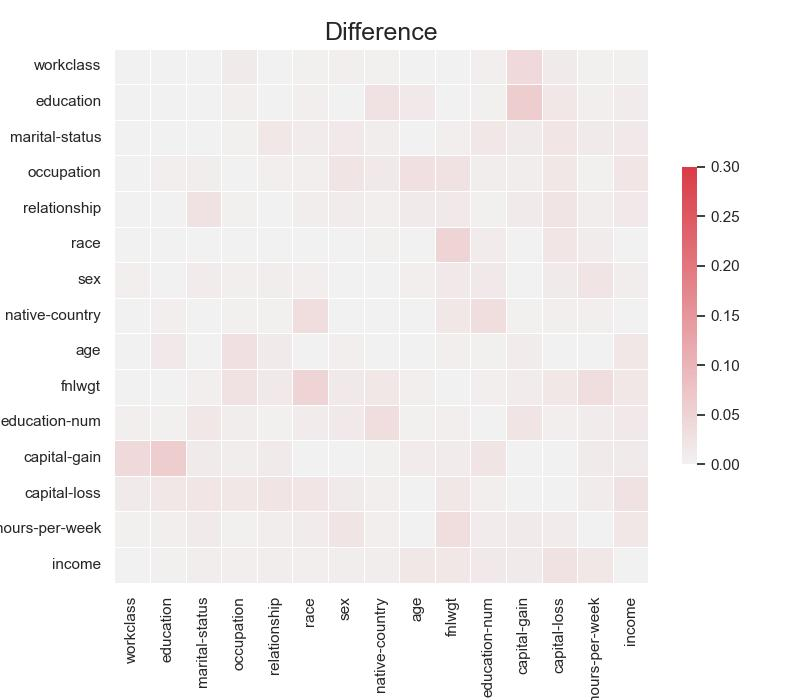
\includegraphics[width=\textwidth]{images/correlation_difference/tab-ddpm-bgm.jpg}
		\caption{TabDDPM-BGM$^{ml}_q$}
	\end{subfigure}
	\hfill
	\begin{subfigure}{0.3\textwidth}
		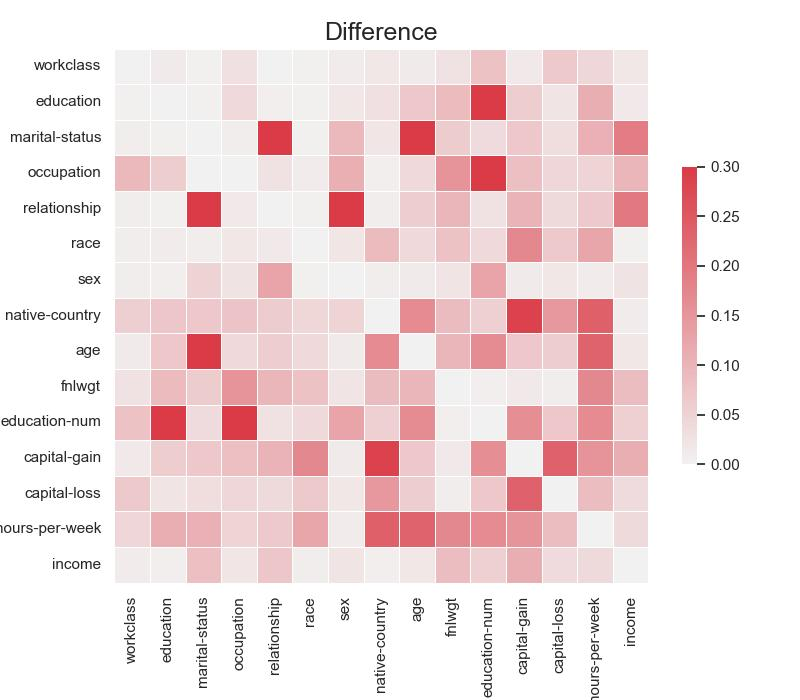
\includegraphics[width=\textwidth]{images/correlation_difference/tab-ddpm-ft.jpg}
		\caption{TabDDPM-FT$^{ml}_q$}
	\end{subfigure}
	\hfill
	\begin{subfigure}{0.3\textwidth}
		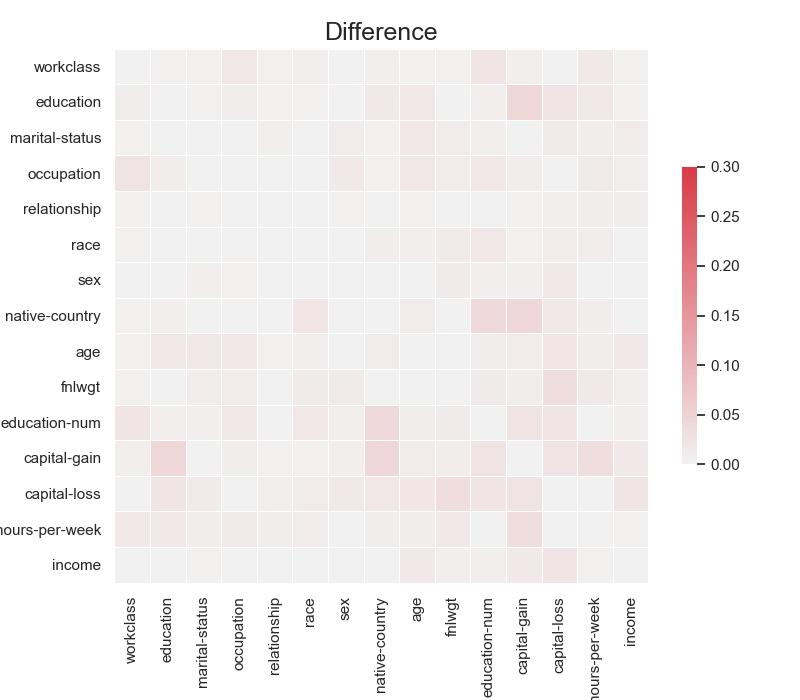
\includegraphics[width=\textwidth]{images/correlation_difference/tab-ddpm-bgm-simTune-minmax.jpg}
		\caption{TabDDPM-BGM$^{s}_m$}
	\end{subfigure}
	\caption{Correlation Matrix difference from selected experiment models.}
	\label{fig:corr_diffusion}
\end{figure}



\autoref{fig:corr_diffusion} shows that while the TabDDPM-BGM$^{ml}$ are able to produce small correlation differences, the TabDDPM-FT$^{ml}$ is not able to reproduce
the correlation matrix of the real dataset.
The overall best correlation difference matrix is produced by TabDDPM$^{s}_m$, which is also reflected in their TabSynDex correlation score in \autoref{tab:exp3-sim}, which is highest across all model versions.
Other model versions matrices do not show any noteworthy changes and are displayed in \autoref{fig_a:corr_diff}.

\subsection[]{Principle Component Analysis}
\label{ch:results-pca}

A \gls{pca} is a dimensionality reduction technique, that converts a dataset onto principal components \cite{brenninkmeijer2019GenerationEvaluationTabular}.
The components are then sorted according to the amount of variance from the original dataset each component is able to capture.
The following visualizations map the first two principal components, \ie the components that capture the most variance from data.


\begin{figure}[h]
	\centering
	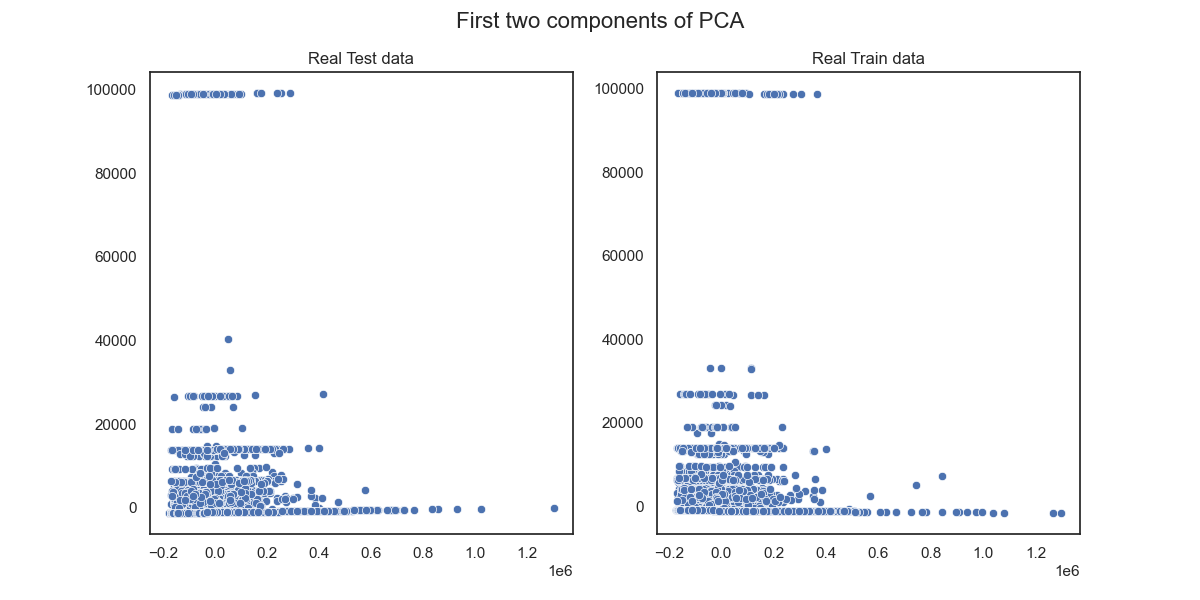
\includegraphics[width=0.6\textwidth]{images/pca/pca.png}
	\caption{\gls{pca} for the real training and testing dataset}
	\label{fig:pca}
\end{figure}

\autoref{fig:pca} shows the two \gls{pca} plots that display the fist two principle components from the real training and testing dataset.
One can see that the majority of values in the plots are scatter around the lower left corner (for $y<=40000$) with two accumulations of values spreading along the $x$-axis around $y=100000$ and $y=0$.
The goal of the synthetic data generation method is to produce synthetic data whose \gls{pca} plot is similar to the \gls{pca} plot of the real testing dataset.

\begin{figure}[h]
	\centering
	\begin{subfigure}{0.3\textwidth}
		\centering
		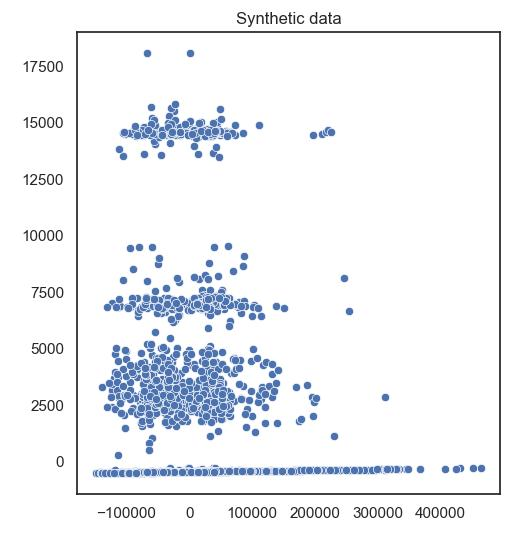
\includegraphics[width=\textwidth]{images/pca/tvae.jpg}
		\caption{TVAE$^{ml}$}
	\end{subfigure}
	\begin{subfigure}{0.3\textwidth}
		\centering
		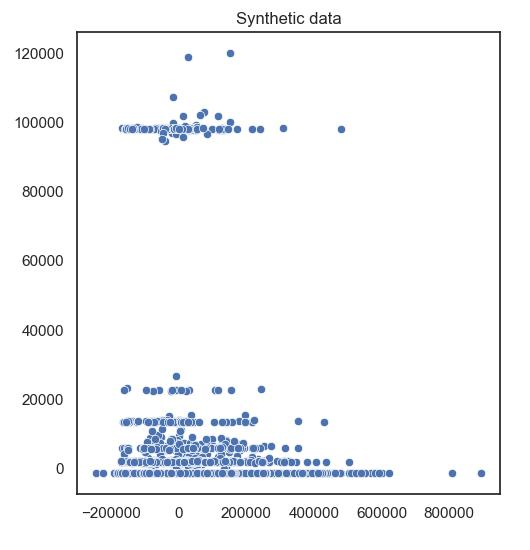
\includegraphics[width=\textwidth]{images/pca/ctabgan.jpg}
		\caption{CTABGAN$^{ml}$}
	\end{subfigure}
	\begin{subfigure}{0.3\textwidth}
		\centering
		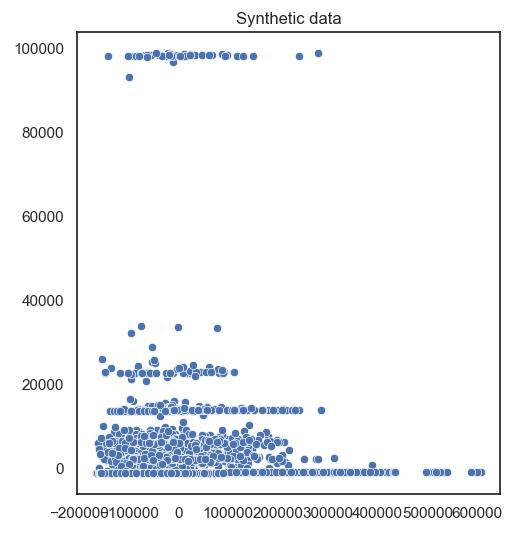
\includegraphics[width=\textwidth]{images/pca/ctabgan+.jpg}
		\caption{CTABGAN+$^{ml}$}
	\end{subfigure}
	\begin{subfigure}{0.3\textwidth}
		\centering
		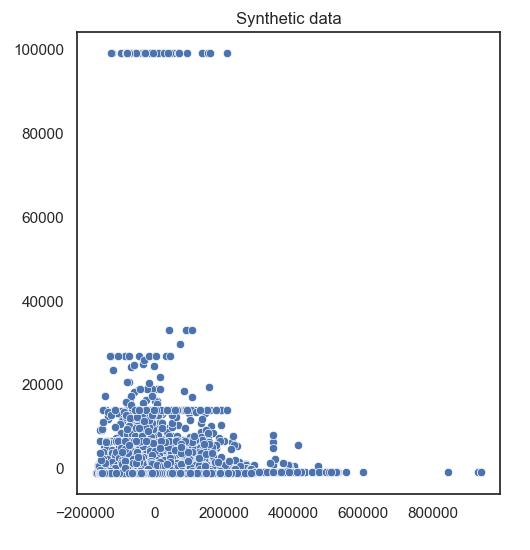
\includegraphics[width=\textwidth]{images/pca/smote.jpg}
		\caption{SMOTE}
	\end{subfigure}
	\begin{subfigure}{0.3\textwidth}
		\centering
		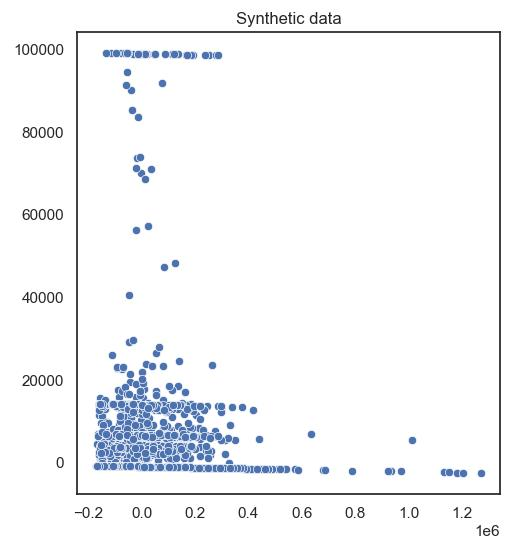
\includegraphics[width=\textwidth]{images/pca/tab-ddpm.jpg}
		\caption{TabDDPM$^{ml}_q$}
	\end{subfigure}
	\caption{\gls{pca} for Baseline models.}
	\label{fig:pca_base}
\end{figure}

\autoref{fig:pca_base} shows the \gls{pca} plots for the different baseline models. All plots show some similarity with the \gls{pca}-plot from the original dataset,
except for the TVAE model.

\begin{figure}[H]
	\centering
	\begin{subfigure}{0.23\textwidth}
		\centering
		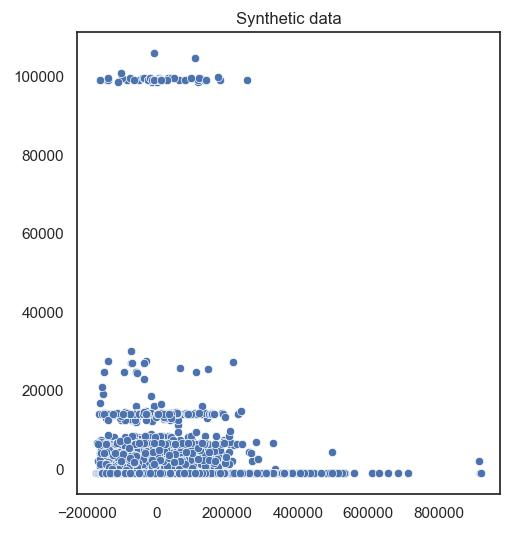
\includegraphics[width=\textwidth]{images/pca/tab-ddpm-bgm.jpg}
		\caption{TabDDPM-BGM$^{ml}_q$}
	\end{subfigure}
	\begin{subfigure}{0.23\textwidth}
		\centering
		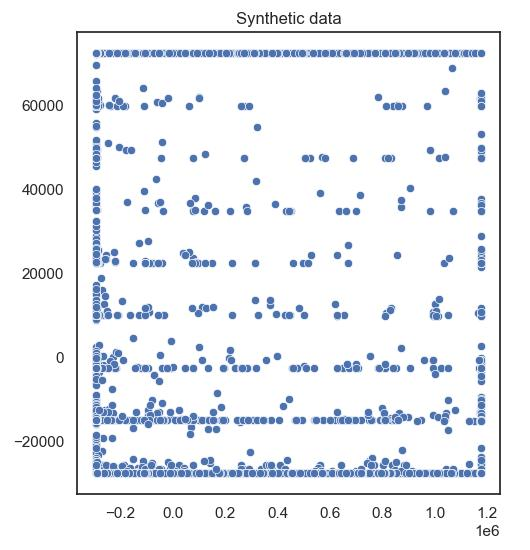
\includegraphics[width=\textwidth]{images/pca/tab-ddpm-ft.jpg}
		\caption{TabDDPM-FT$^{ml}_q$}
	\end{subfigure}
	\begin{subfigure}{0.23\textwidth}
		\centering
		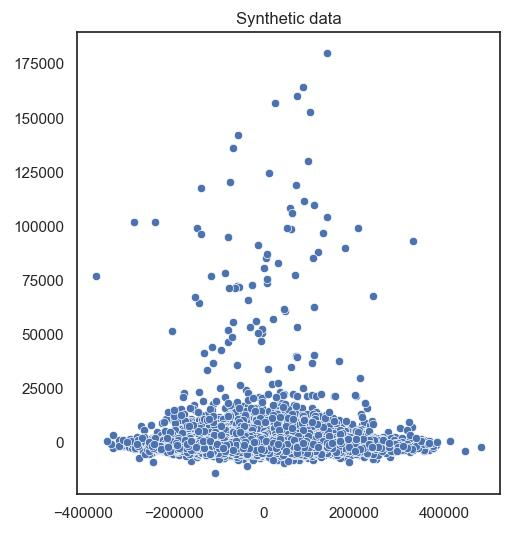
\includegraphics[width=\textwidth]{images/pca/tab-ddpm-simTune-minmax.jpg}
		\caption{TabDDPM$^{s}_m$}
	\end{subfigure}
	\begin{subfigure}{0.23\textwidth}
		\centering
		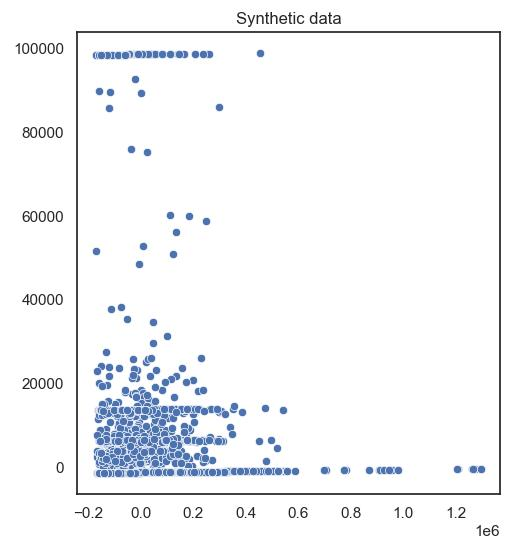
\includegraphics[width=\textwidth]{images/pca/tab-ddpm-simTune.jpg}
		\caption{TabDDPM$^{s}_q$}
	\end{subfigure}
	\caption{\gls{pca} for selected experiment models.}
	\label{fig:pca_diffusion}
\end{figure}

Only the \gls{bgm} tabular processing mechanism seems to be able to produce a realistic \gls{pca}-plot.
Additionally, the Minmax scaling seems to have an effect on the \gls{pca}-plot for the TabDDPM model, however,
this did not affect the TabDDPM-BGM model that made use of Minmax scaling (\autoref{fig_a:pca_TabDDPMBM}).
This \gls{pca}-plot and the remaining model versions plots can be found at \autoref{A:pca}.

\subsection[]{Distribution Plot}
\label{ch:results-Distr}

For each model version distribution plots for each column can be found at \autoref{A:distributions}, comparing the distributions of the synthetic data with the real data.
This section will highlight some interesting plots for selected models.

In terms of categorical distributions (\autoref{fig:education} displays the education column distributions as an example) all baseline models are able to reproduce the original distributions,
with CTABGAN+$^{ml}$ and TabDDPM$^{ml}_q$ replicating the original distribution best.
The \gls{bgm} tabular processing model also reproduced the categorical distributions in a comparable way to the TabDDPM counterpart.
The \gls{ft} tabular processing model on the other hand, was not able reproduce the original distribution at all and failed to mimic the real data.

\begin{figure}[h]
	\centering
	\begin{subfigure}{0.23\textwidth}
		\centering
		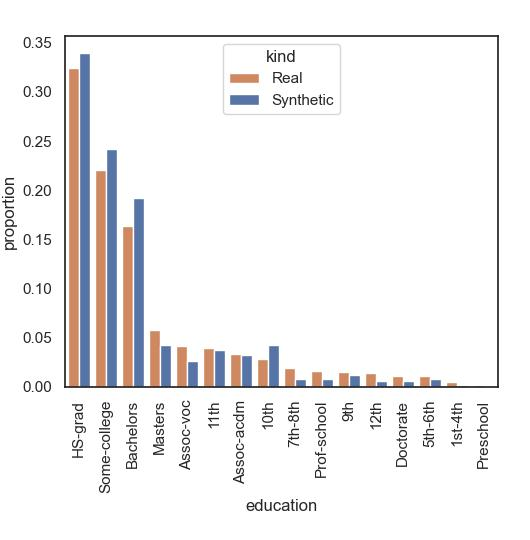
\includegraphics[width=\textwidth]{images/dist_education/tvae.jpg}
		\caption{TVAE$^{ml}$}
	\end{subfigure}
	\begin{subfigure}{0.23\textwidth}
		\centering
		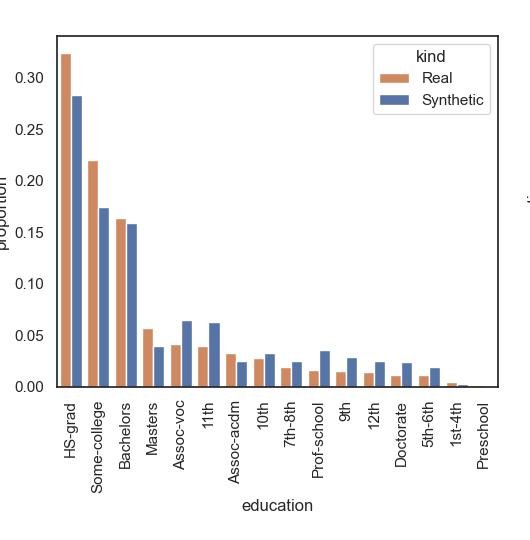
\includegraphics[width=\textwidth]{images/dist_education/ctabgan.jpg}
		\caption{CTABGAN$^{ml}$}
	\end{subfigure}
	\begin{subfigure}{0.23\textwidth}
		\centering
		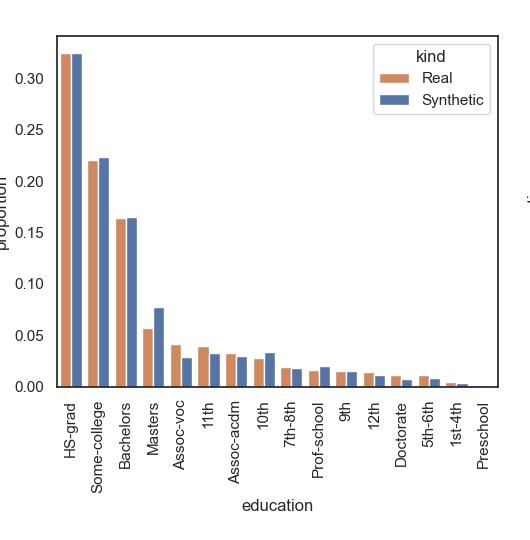
\includegraphics[width=\textwidth]{images/dist_education/ctabgan+.jpg}
		\caption{CTABGAN+$^{ml}$}
	\end{subfigure}
	\begin{subfigure}{0.23\textwidth}
		\centering
		\includegraphics[width=\textwidth]{images/dist_education/SMOTE.jpg}
		\caption{SMOTE}
	\end{subfigure}
	\begin{subfigure}{0.23\textwidth}
		\centering
		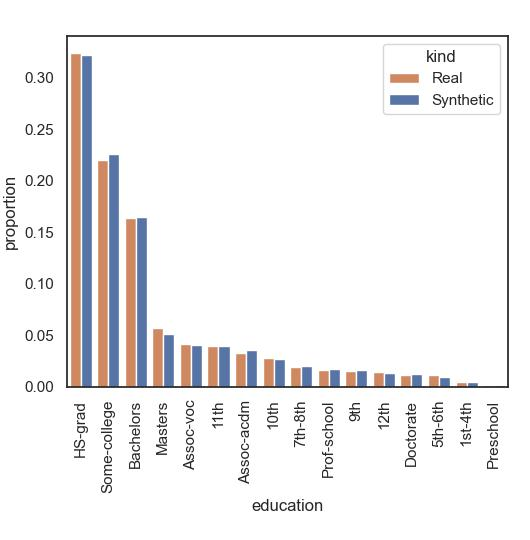
\includegraphics[width=\textwidth]{images/dist_education/tab-ddpm.jpg}
		\caption{TabDDPM$^{ml}_q$}
	\end{subfigure}
	\begin{subfigure}{0.23\textwidth}
		\centering
		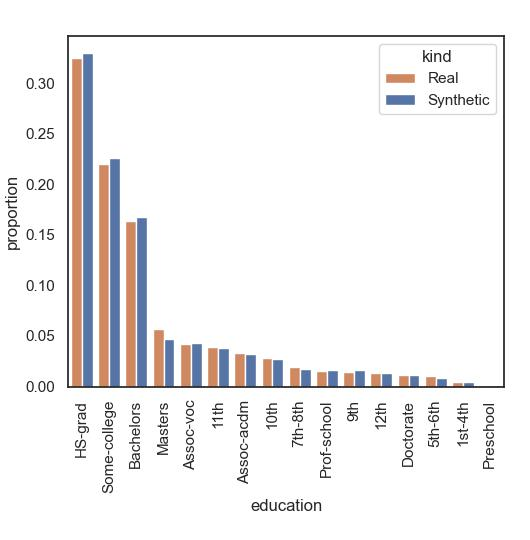
\includegraphics[width=\textwidth]{images/dist_education/tab-ddpm-bgm.jpg}
		\caption{TabDDPM-BGM$^{ml}_q$}
	\end{subfigure}
	\begin{subfigure}{0.23\textwidth}
		\centering
		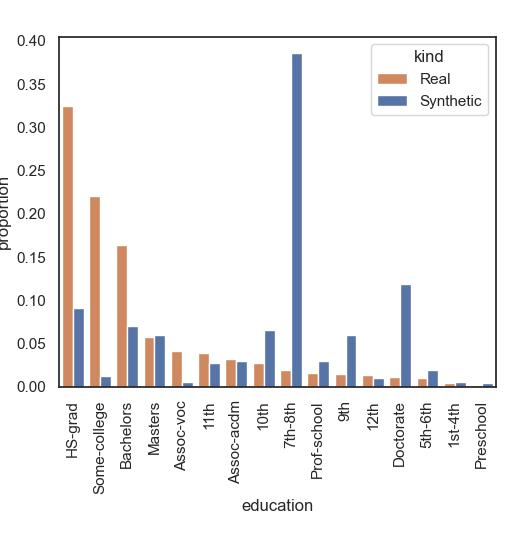
\includegraphics[width=\textwidth]{images/dist_education/tab-ddpm-ft.jpg}
		\caption{TabDDPM-FT$^{ml}_q$}
	\end{subfigure}
	\caption{Education column for baseline models.}
	\label{fig:education}
\end{figure}

The tuning towards the similarity score did not affect the categorical distributions in any model.
The same is true for changing to the Minmax scaling, since it only affects continuous values.


\begin{figure}[h]
	\centering
	\begin{subfigure}{0.23\textwidth}
		\centering
		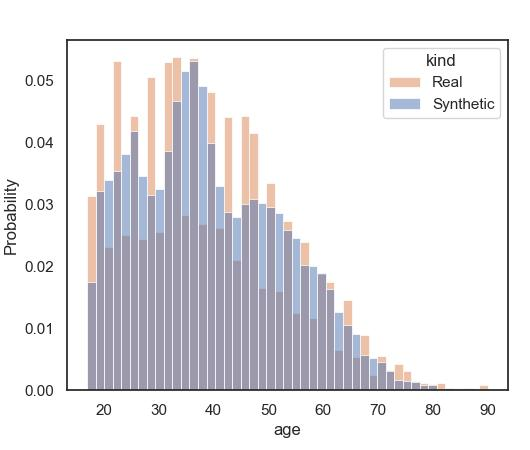
\includegraphics[width=\textwidth]{images/dist_age/tvae.jpg}
		\caption{TVAE$^{ml}$}
	\end{subfigure}
	\begin{subfigure}{0.23\textwidth}
		\centering
		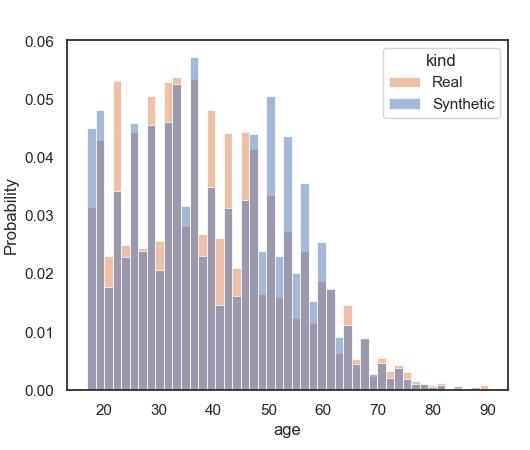
\includegraphics[width=\textwidth]{images/dist_age/ctabgan.jpg}
		\caption{CTABGAN$^{ml}$}
	\end{subfigure}
	\begin{subfigure}{0.23\textwidth}
		\centering
		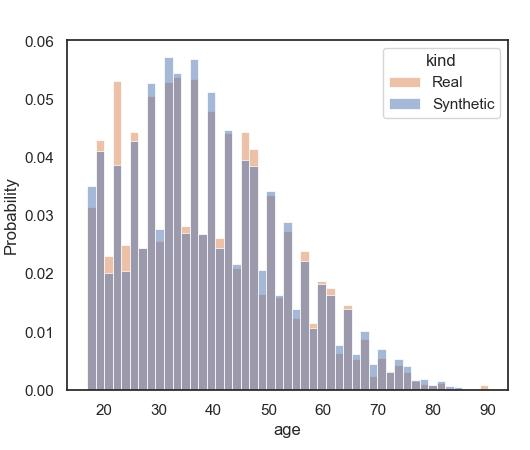
\includegraphics[width=\textwidth]{images/dist_age/ctabgan+.jpg}
		\caption{CTABGAN+$^{ml}$}
	\end{subfigure}
	\begin{subfigure}{0.23\textwidth}
		\centering
		\includegraphics[width=\textwidth]{images/dist_age/SMOTE.jpg}
		\caption{SMOTE}
	\end{subfigure}
	\begin{subfigure}{0.23\textwidth}
		\centering
		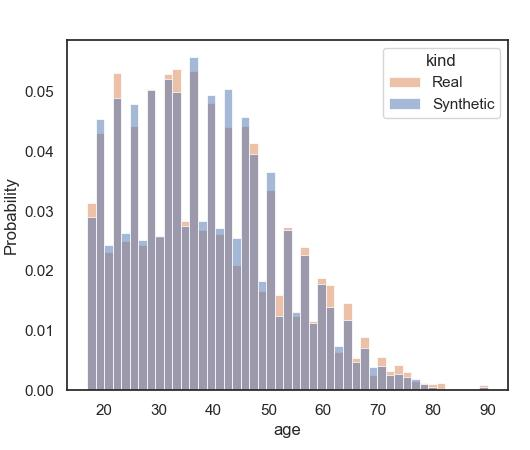
\includegraphics[width=\textwidth]{images/dist_age/tab-ddpm.jpg}
		\caption{TabDDPM$^{ml}_q$}
	\end{subfigure}
	\begin{subfigure}{0.23\textwidth}
		\centering
		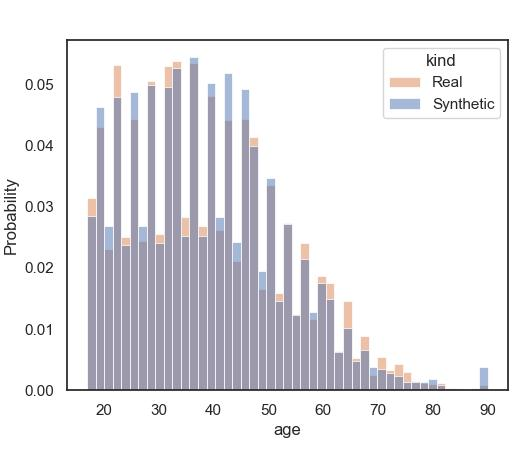
\includegraphics[width=\textwidth]{images/dist_age/tab-ddpm-simTune.jpg}
		\caption{TabDDPM$^{s}_q$}
	\end{subfigure}
	\begin{subfigure}{0.23\textwidth}
		\centering
		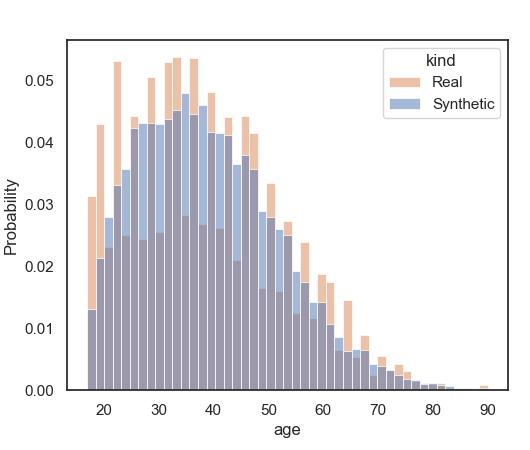
\includegraphics[width=\textwidth]{images/dist_age/tab-ddpm-simTune-minmax.jpg}
		\caption{TabDDPM$^{s}_m$}
	\end{subfigure}
	\begin{subfigure}{0.23\textwidth}
		\centering
		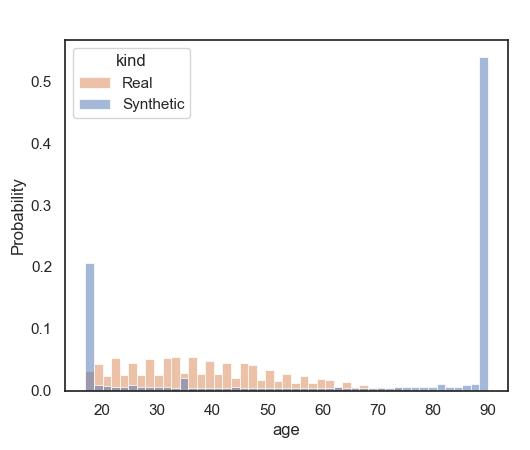
\includegraphics[width=\textwidth]{images/dist_age/tab-ddpm-ft.jpg}
		\caption{TabDDPM-FT$^{ml}_q$}
	\end{subfigure}
	\begin{subfigure}{0.23\textwidth}
		\centering
		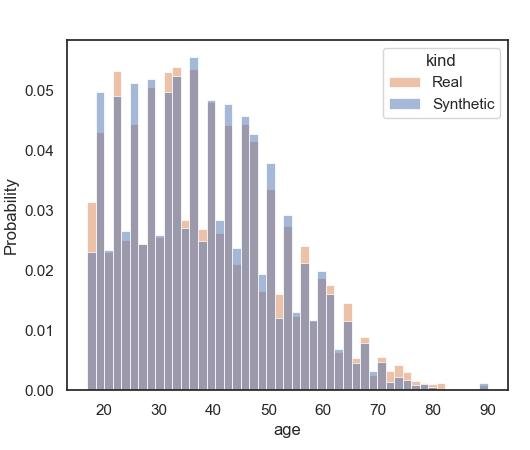
\includegraphics[width=\textwidth]{images/dist_age/tab-ddpm-bgm.jpg}
		\caption{TabDDPM-BGM$^{ml}_q$}
	\end{subfigure}
	\begin{subfigure}{0.23\textwidth}
		\centering
		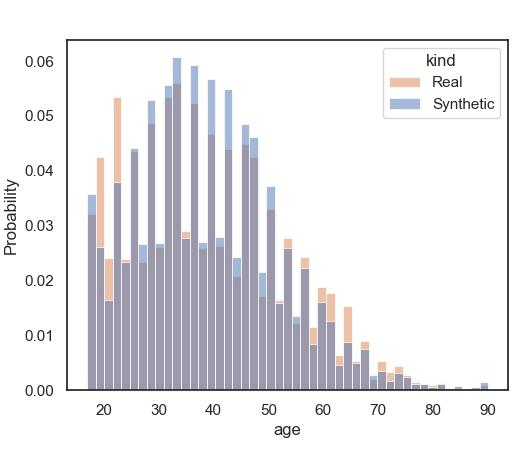
\includegraphics[width=\textwidth]{images/dist_age/tab-ddpm-bgm-simTune-minmax.jpg}
		\caption{TabDDPM-BGM$^{s}_m$}
	\end{subfigure}
	\caption{Age column for selected model versions. Please note, that the Y-axis range may vary due to the range of the synthetic data.}
	\label{fig:age}
\end{figure}

\autoref{fig:age} shows, that this observation does not extend towards continuos columns, given the column age as an example.
Across the baseline models, CTABGAN+$^{ml}$ and TabDDPM$^{ml}_q$ are again best able to reproduce the original data distribution of the example column.
All TabDDPM-BGM models produce distributions, that are comparable to those produced by the baseline TabDDPM.
Again, TabDDPM-FT, fails to replicate the target distributions at all.
Interestingly, the similarity score hyperparameter optimization did not affect the TabDDPM distributions to any visible extend.
However, the Minmax scaling reduced the TabDDPM capability to create a realistic distribution, whose probability distributions rather follows a Gaussian distribution, failing to replicate the detailed peaks of the original dataset.
This behavior was not present in the \gls{bgm} version with Minmax scaling.


\subsection[]{Cumulative distribution function}

All \gls{cdf} plots can be found in \autoref{A:cumsum}.
The plots show, that the \glspl{cdf} of the synthetic data created by CTABGAN+$^{ml}$ and TabDDPM$^{ml}_q$ comes closest to
the \glspl{cdf} of the real data across the baseline models (best visible for columns "native-country" or "hours-per-week").
The selected plots in \autoref{fig:cdf} show how the \gls{ft} tabular processing failed again to reproduce the original datas \gls{cdf}.
TabDDPM-BGM on the other hand was able to produce synthetic data, whose \gls{cdf} correctly mimics the \gls{cdf} of the real data.
One could argue, that TabDDPM and TabDDPM that have been tuned after the similarity score are slightly better able to
reproduce \gls{cdf} plots for categorical columns whose categories are imbalanced (\eg see column "native-country", where the majority of values equal "United-States").
This improvement is more visible for the \gls{bgm} version.
The Minmax scaling did affect the TabDDPM version greatly and "smoothed out" its \glspl{cdf}.
This phenomenon was not present in the TabDDPM-BGM version with Minmax scaling.


\begin{figure}[H]
	\centering
	\begin{subfigure}{0.23\textwidth}
		\centering
		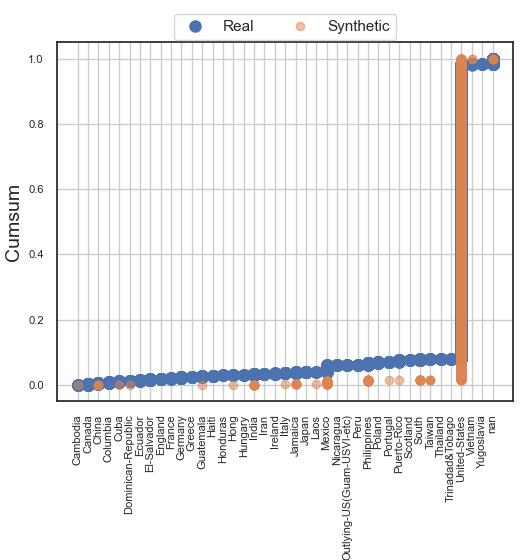
\includegraphics[width=\textwidth]{images/cdf/tvae.jpg}
		\caption{TVAE$^{ml}$}
	\end{subfigure}
	\begin{subfigure}{0.23\textwidth}
		\centering
		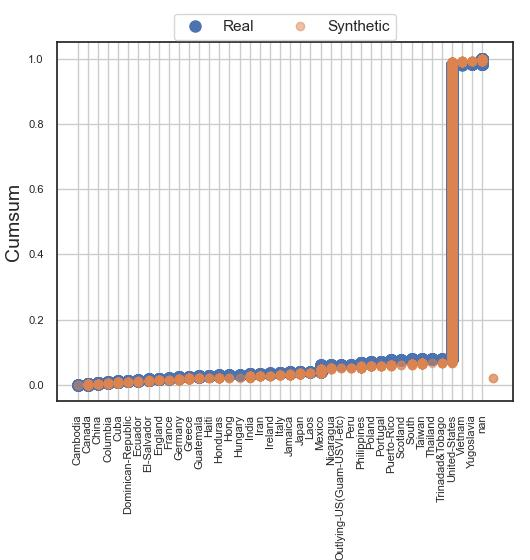
\includegraphics[width=\textwidth]{images/cdf/ctabgan+.jpg}
		\caption{CTABGAN+$^{ml}$}
	\end{subfigure}
	\begin{subfigure}{0.23\textwidth}
		\centering
		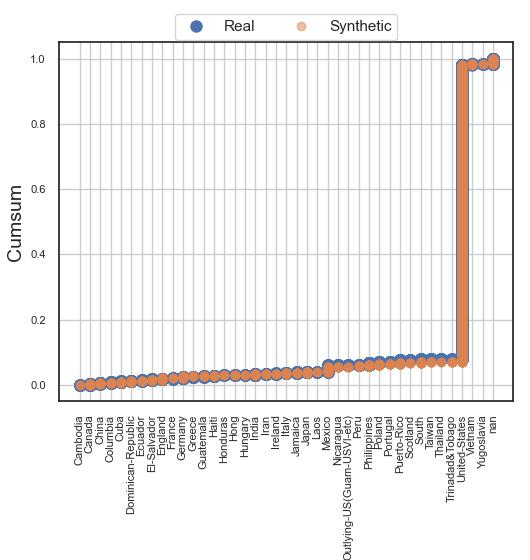
\includegraphics[width=\textwidth]{images/cdf/tab-ddpm-bgm-simTune.jpg}
		\caption{TabDDPM-BGM$^{s}_q$}
	\end{subfigure}
	\begin{subfigure}{0.23\textwidth}
		\centering
		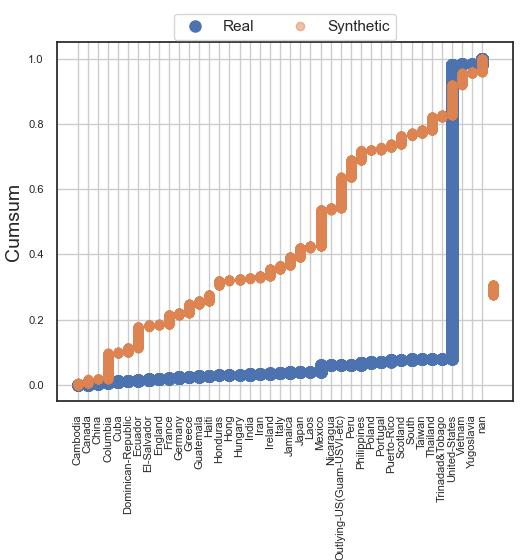
\includegraphics[width=\textwidth]{images/cdf/tab-ddpm-ft.jpg}
		\caption{TabDDPM-FT$^{ml}_q$}
	\end{subfigure}
	\begin{subfigure}{0.23\textwidth}
		\centering
		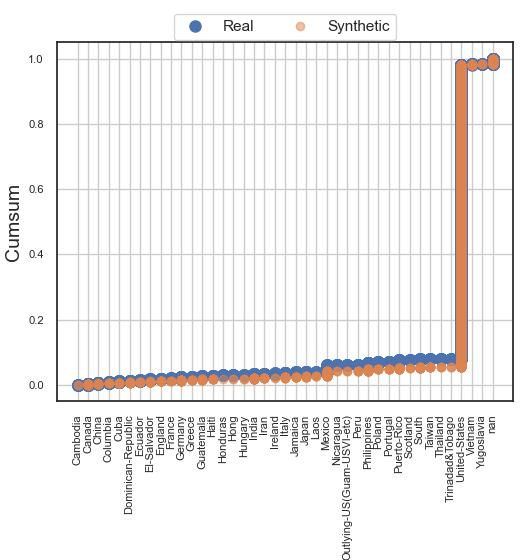
\includegraphics[width=\textwidth]{images/cdf/tab-ddpm.jpg}
		\caption{TabDDPM$^{ml}_q$}
	\end{subfigure}
	\begin{subfigure}{0.23\textwidth}
		\centering
		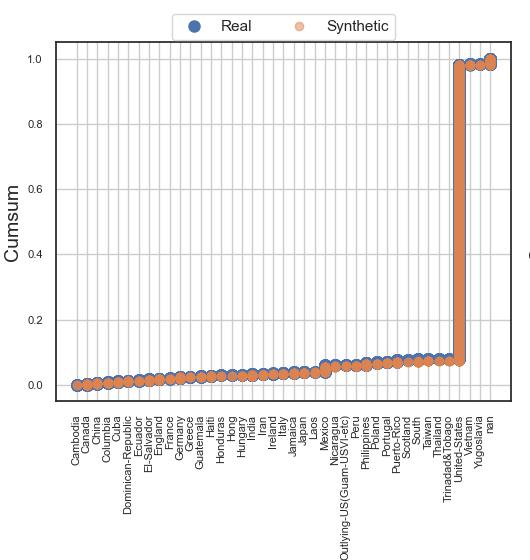
\includegraphics[width=\textwidth]{images/cdf/tab-ddpm-simTune-minmax.jpg}
		\caption{TabDDPM$^{s}_m$}
	\end{subfigure}
	\caption{\gls{cdf} plots for selected model versions for the columns "native-country" and "hours-per-week" of the adult income dataset \cite{Dua:2019}}
	\label{fig:cdf}
\end{figure}



\newpage

\section{Discussion}
\label{ch:results-discussion}
%-------------------------------------------------------------------------

The goal of this thesis is to investigate the performance of adding the tabular processing mechanisms to the TabDDPM model (\gls{rq}1) and 
to expand upon the already existing machine learning efficacy evaluation performed by \cite{kotelnikov2022TabDDPMModellingTabular} through the similarity score metrics proposed by \cite{chundawat2022UniversalMetricRobust}.

\subsection*{Analysis of Visual and Numerical Results}

\begin{table}[h]
	\centering
	\begin{tabular}{lrrr}
		\toprule
		\textbf{Model}       & \textbf{Accurarcy} & \textbf{F1}     & \textbf{ROC-AUC} \\
		\midrule
		Real                 & 0.874              & 0.815           & 0.928            \\
		TVAE$^{ml}$          & 0.845              & 0.780           & 0.900            \\
		SMOTE                & 0.858              & 0.791           & 0.910            \\
		CTABGAN$^{ml}$       & 0.850              & 0.775           & 0.900            \\
		CTABGAN+$^{ml}$      & 0.855              & 0.775           & 0.907            \\
		TabDDPM$^{ml}_q$     & 0.860              & 0.794           & 0.913            \\
		TabDDPM-BGM$^{ml}_q$ & \textbf{0.863}     & \textbf{0.798} & \textbf{0.916}   \\
		TabDDPM-FT$^{ml}_q$  & 0.785              & 0.552           & 0.821            \\
		CTABGAN$^{s}_q$      & 0.850              & 0.776           & 0.900            \\
		TVAE$^{s}$           & 0.845              & 0.780           & 0.900            \\
		TabDDPM$^{s}_q$      & 0.856              & 0.782           & 0.908            \\
		TabDDPM-BGM$^{s}_q$  & 0.859              & 0.792           & 0.911            \\
		TabDDPM-FT$^{s}_q$   & 0.766              & 0.451           & 0.712            \\
		TabDDPM$^{s}_m$      & 0.856              & 0.778           & 0.910            \\
		TabDDPM-BGM$^{s}_m$  & 0.857              & 0.787           & 0.909            \\
		\bottomrule
	\end{tabular}
	\caption[]{Overview of all CatBoost machine learning efficacy results for all tested model versions.}
	\label{tab:ml-all}
\end{table}


\begin{table}[h]
	\centering
	\begin{tabular}{lrrrrrr}
		\toprule
		\textbf{Model}       & \textbf{Similarity Score} & \textbf{Basic} & \textbf{Correlation} & \textbf{ML}    & \textbf{Support} & \textbf{pMSE}  \\
		\midrule
		Real                 & 0.960                     & 0.992          & 0.943                & 0.998          & 0.984            & 0.882          \\
		TVAE$^{ml}$          & 0.658                     & 0.854          & 0.814                & 0.962          & 0.657            & 0.000          \\
		SMOTE                & 0.723                     & 0.953          & 0.865                & 0.992          & 0.804            & 0.000          \\
		CTABGAN$^{ml}$       & 0.741                     & 0.940          & 0.832                & 0.984          & 0.947            & 0.000          \\
		CTABGAN+$^{ml}$      & 0.750                     & 0.969          & 0.882                & 0.990          & 0.892            & 0.019          \\
		TabDDPM$^{ml}_q$     & 0.759                     & 0.973          & 0.919                & 0.992          & 0.874            & 0.035          \\
		TabDDPM-BGM$^{ml}_q$ & 0.742                     & 0.964          & 0.918                & \textbf{0.996} & 0.831            & 0.000          \\
		TabDDPM-FT$^{ml}_q$  & 0.595                     & 0.495          & 0.648                & 0.869          & 0.963            & 0.000          \\
		CTABGAN$^{s}_q$      & 0.740                     & 0.938          & 0.833                & 0.984          & 0.947            & 0.000          \\
		TVAE$^{s}$           & 0.658                     & 0.856          & 0.815                & 0.962          & 0.656            & 0.000          \\
		TabDDPM$^{s}_q$      & 0.852                     & 0.976          & 0.921                & 0.991          & 0.952            & 0.420          \\
		TabDDPM-BGM$^{s}_q$  & 0.857                     & \textbf{0.982} & 0.858                & 0.991          & 0.920            & 0.532          \\
		TabDDPM-FT$^{s}_q$   & 0.588                     & 0.512          & 0.619                & 0.818          & \textbf{0.992}   & 0.000          \\
		TabDDPM$^{s}_m$      & \textbf{0.869}            & 0.938          & \textbf{0.930}       & 0.990          & 0.928            & \textbf{0.558} \\
		TabDDPM-BGM$^{s}_m$  & 0.856                     & 0.981          & 0.913                & 0.992          & 0.915            & 0.476          \\
		\bottomrule
	\end{tabular}
	\caption[]{Overview of all similarity score results for all tested model versions.}
	\label{tab:sim-all}
\end{table}
[TODO: Tune ctabgan+]

Based on the obtained results, it is evident that the processing mechanism for \gls{ft} has failed and is not advisable. 
Despite having the highest overall support score, all other measurements and visual representations indicate that the model was not capable of generating synthetic data that closely resembles the original dataset.
As a consequence, the TabDDPM-FT variations will not be further discussed and analyzed.
The \gls{bgm} processor variant was able to produce not only good numerical but also visual results.
In terms of machine learning efficacy, the TabDDPM-BGM$^{ml}_q$ version shows the best machine learning efficacy performance across all tested metrics (\autoref{tab:ml-all}: Accurarcy, F1 and AUC-ROC and \autoref{tab:sim-all}: ML).
However, the advantage over its simpler counterpart TabDDPM$^{ml}_q$ is only marginal (+0.003\%-points).
Overall, models with hyperparameters tuned towards machine learning efficacy outperform models with hyperparameters tuned towards similarity score in the machine learning efficacy scores, as one would expect.
For the non-diffusion baseline models, the results show, that the SMOTE approach is a reliable sampling technique when the synthetic data will be used in a machine learning scenario.
Its machine learning efficacy results are superior to the other non-diffusion baseline models while the model being overall less complex.
For other scenarios, CTABGAN+ achieves the best overall performance in terms of numerical and visual results, for non-diffusion based models.
Nevertheless, the best found CTABGAN+ version is inferior to the best found diffusion model [TODO: Check].

Changing the tuning strategy to the similarity score, allowed several observations to be made.
Firstly, non-diffusion models metric results had no significant effects on the baseline models, all of their metric scores stayed roughly the same.
Diffusion models on the other hand, showed several changes in the numerical results.
Overall, diffusion models with a similarity score tuning show reduced machine learning efficacy metric scores compared to their machine learning efficacy counterpart.
While this reduction is relative small, the similarity metrics have been increased significantly.
Especially the \gls{pmse} score was increased (+0.4-0.5\%-points), thanks to the similarity tuning.
% Sim Tune - pmse
The big increase in the \gls{pmse} score for diffusion models is especially worth highlighting.
Previously, all non-diffusion baseline models failed to produce data, that is non-differentiable from the real-data by a logistic regression model, which is indicated by the \gls{pmse} score.
This confirms the observation made by the authors of \cite{chundawat2022UniversalMetricRobust}, who also observe that all of their tested models (mainly \gls{gan}-based) achieve a \gls{pmse} of 0.
\cite{chundawat2022UniversalMetricRobust} experiments only identified one model, a \gls{gan} model with gradient penalty and wasserstein distance, which was able to achieve a peak \gls{pmse} score of 0.4.
Tuning the hyperparameter towards the similarity score, which includes the \gls{pmse} score, allows to increase the \gls{pmse} score to values between 0.42 and 0.55 for diffusion models TabDDPM and TabDDPM-BGM.
The same tuning strategy did not affect the \gls{pmse} score of baseline models like TVAE or CTABGAN. 
This indicates that diffusion based models are better able to produce synthetic data, that is harder to differentiate from its real counterpart.

In addition to the increase of the \gls{pmse} score, the other metrics that make up the similarity score have increased as well, but on a smaller scale.
Only correlation values got decreased slightly through the similarity tuning.
This observation holds for TabDDPM and TabDDPM-BGM, but not for the baseline models (TVAE and CTABGAN), whose metric results remained unchanged after switching the tuning strategy..
This indicates, that the importance for hyperparameter tuning is much higher for diffusion models in tabular data synthesis, as their tuning strategy affects the metric outcomes significantly.

Replacing the quantile transform function with minmax scaling for the TabDDPM (TabDDPM$^{s}_m$) has led to the highest overall similarity score.
It scored highest in both correlation and \gls{pmse}, leading to the high overall similarity score.
According to \cite{QuantileTransformer}, the quantile transform function is a non-linear transformation that may distort correlations between variables.
This is also observable in the correlation metric score, where TabDDPM$^{s}_q$ and TabDDPM-BGM$^{s}_q$ have a lower correlation score than their minmax scaling counterpart.
However, it is important to also take into consideration the visual results.
Although the correlation difference plot of TabDDPM$^{s}_m$ appears satisfactory, the distribution and \gls{cdf} plot of continuous columns look worse when compared to those of other models. 
The continuous plots of TabDDPM$^{s}_m$ lack details and rather approximate the original distribution.
The models quantile transform counterpart TabDDPM$^{s}_q$ does not show this behavior, producing overall more realistic plots.
This indicates that the minmax scaling, which is applied to the numerical columns, causes this kind of behavior.
On the other hand, TabDDPM-BGM$^{s}_m$, does not show this behavior even though MinMax scaling is applied. 
However for TabDDPM-BGM, after the MinMax is inverted, the tabular processing mechanism is inverted as well, which involves the mode-specific normalization in the case of the \gls{bgm}-Processor.
This indicates, that the TabDDPM-BGM is not affected by quantile or minmax scaling to the same extend, as the plain TabDDPM is.

To summarize, the following observations could be made:

\begin{itemize}
	\item The processing mechanism for \gls{ft} has failed and is not advisable, as it could not generate synthetic data that closely resembles the original dataset.
	\item The \gls{bgm} processor produced good numerical and visual results.
	\item TabDDPM-BGM$^{ml}_q$ shows the best machine learning efficacy performance across all tested metrics.
	\item Out of the baseline models, SMOTE is a reliable sampling technique for non-diffusion baseline models in machine learning scenarios.
	In other scenarios, CTABGAN+ is the preferred non-diffusion model.
	\item Diffusion models outperform non-diffusion models in tabular data synthesis.
	\item Diffusion models with similarity score tuning led to models with an non-zero \gls{pmse} score.
	\item Hyperparameter tuning is more important for diffusion models in tabular data synthesis, as their tuning strategy significantly affects metric outcomes.
	\item Replacing the quantile transform function with minmax scaling for TabDDPM (TabDDPM$^{s}_m$) led to the highest overall similarity score, but also resulted in worse distribution and \gls{cdf} plot of continuous columns.
	\item TabDDPM-BGM is not affected by quantile or minmax scaling to the same extent as the plain TabDDPM.
\end{itemize}

\subsection*{Analysis of Research Questions}

\subsubsection{RQ1}

The results obtained in this study provide insights into the research questions posed in Section \ref{ch:intro-goals}.
\gls{rq}1 is concerned with the effects of additional tabular data processing mechanisms on TabDDPM.
It could be shown, that by incorporating additional tabular data processing mechanisms, the TabDDPM model was able to achieve improved performance compared to the baseline models.
This was only the case for the \gls{bgm} processing but not the \gls{ft} processing.
It was found that the TabDDPM-BGM$^{s}_q$ is the best suited model for producing synthetic data, that will be used in a machine learning scenario.
Even though TabDDPM$^{s}_m$ achieved the highest overall similarity score, its visual results lack detail for numerical columns.
Hence TabDDPM-BGM should in general be preferred, with TabDDPM-BGM$^{s}_q$ producing slightly better basic, support and \gls{pmse} scores and TabDDPM-BGM$^{s}_m$ producing good correlations.

The visual results reinforced these findings, with correlation difference and PCA plots produced by TabDDPM-BGM variants closely resembling the original dataset.
In addition to that, TabDDPM-BGM are reliably able to reproduce distributions and \glspl{cdf} of the original dataset.
The biggest difference was observable when replacing the quantile transformation with the minmax scaling.
While the plain TabDDPM$^s_m$ model struggled to reproduce the detail in the original continuos columns, the \gls{bgm} processing variant was able to.

To summarize, the tabular processor encodes the data into a different data format, which will be processed by the TabDDPM afterwards.
Depending on the encoded data format, the generative capability of TabDDPM changed.
From the \gls{ft} processed data, the TabDDPM model was not able to generate realistic synthetic data.
The \gls{bgm} technique on the other hand, encoded the data in a reliable manner, such that the diffusion model was able to produce synthetic data, that closely resemblance the original dataset in multiple aspects.
With the \gls{bgm} technique, the TabDDPM showed improved generative capabilities, with better performance across various metrics and more realistic synthetic data generation, compared to TabDDPM without \gls{bgm}.
Hence, the results suggest, that introducing a tabular processor to the synthesization pipeline can improve the overall quality of the produce synthetic data.


\subsubsection{RQ2}
\gls{rq}2 is concerned with an extended evaluation of Diffusion based tabular data synthesis, that goes beyond an machine learning efficacy evaluation.
In this thesis, TabSynDex evaluation metric \cite{chundawat2022UniversalMetricRobust} in addition to a CatBoost machine learning efficacy was performed.
This evaluation revealed new insights into the performance of diffusion based models compared to other model types in tabular data synthesis.
Overall, it could be observed, that the the superior performance of TabDDPM compared to the non-diffusion models found in \cite{kotelnikov2022TabDDPMModellingTabular}
could not only be confirmed with the results of this thesis, but it could be shown that the superior performance also extends to the other tested metrics (basic statistics, correlations, ml, support).

Furthermore, the evaluation also highlights the importance of hyperparameter tuning for diffusion model in tabular data synthesis.
While a change in the hyperparameter tuning strategy did hardly effect non-diffusion models, it greatly effected the TabDDPM approach.  
If hyperparameter are tuned towards the TabSynDex Similarity score, diffusion models outperform all other models, including \gls{vae} and \gls{gan}-based approaches,
in all tested metrics.
The biggest effect was visible in the \gls{pmse} score, indicating the differentiability of the synthetic data from the real data.
Non-diffusion models consistently produced synthetic data, that resulted in a near-zero \gls{pmse} score, even if their hyperparameters have been tuned towards maximizing it.
However, diffusion model variants tested in this thesis were able to produce \gls{pmse} scores of up to 0.55\%.

The evaluation strategy in this thesis also included analysis of visualizations of the synthetic data in multiple ways.
This evaluation revealed, that TabDDPM and its variance produce synthetic data whose plots resemble the original data plots more closely than the synthetic data plots of non-diffusion models.
Additionally, the visual inspect revealed the effects of changing the hyperparameter tuning strategy or data preprocessing strategy has on diffusion models.
For example, TabDDPM$^{s}_m$ metrics result suggest that it produces the best model overall to produce synthetic data, as it has the highest overall similarity score.
However, its plots show a reduced capability to accurately recreate continuos columns.

In summary, the evaluation performed in the thesis showed that TabDDPM and its \gls{bgm} variant outperform other generative models, 
including \gls{vae} and \gls{gan}-based approaches, in an extended similarity evaluation based on the TabSynDex metric, 
machine learning efficacy and a visualization analysis.
Hyperparameter tuning greatly affected the performance of diffusion models, and visualizations revealed that diffusion models produce synthetic data that more closely resemble the original data than non-diffusion models.
Ultimately, this thesis showed the importance of an elaborate evaluation of synthetic data, as new insights on the behavior of diffusion models for tabular data synthesis could be gained,
which are of benefit for potential future diffusion based models.
Additionally, such an extended evaluation allows for a holistic view on the produced synthetic data, uncovering strengths and weaknesses from different perspectives.

\section{Limitations}
\label{ch:results-limitations}
%-------------------------------------------------------------------------

This study has some limitations that need to be acknowledged. 
The biggest limitation is, that only one real dataset (the adult dataset \cite{Dua:2019}) to evaluate the performance of different models has been used. 
Therefore, it is possible that some model versions may perform better or worse on other datasets with different characteristics such as size, dimensionality or complexity. 
The reason for this was the limited access to computing resources.
As a consequence, all observations and results made in this thesis only hold for the adult dataset and should not be generalized, until they can be confirmed on multiple datasets.

A second limitation is that during hyperparameter tuning only a fixed set of hyperparameters were tested. 
Therefore, it is possible that some methods may benefit from further optimization or customization.

Furthermore, although the set of evaluation metrics have been larger compared to the original authors \cite{kotelnikov2022TabDDPMModellingTabular},
an additional, even larger evaluation should be considered. 
In particular, privacy and model complexity related metrics have not been considered in this experiment and would likely reveal new valuable insights.

Lastly, diffusion models, like most other deep neural networks, suffer from a lack of interpretability, as they are considered a black-box model \cite{benitez1997AreArtificialNeural}.

\section{Future Work}
\label{ch:results-futureWork}

As the implementation of diffusion models for synthesizing tabular data represents a relatively innovative approach with limited research to date, numerous promising avenues for future investigations exist.
Firstly, to overcome limitations presented in \autoref{ch:results-limitations} a larger set of datasets are required to confirm the results observed in this thesis.
More datasets with diverse characteristics to generalize the findings and identify potential sources of variation or bias

Moreover, incorporating a variety of metrics with diverse perspectives is essential for evaluating the performance and trade-offs of distinct tabular data generation methods. 
This is particularly relevant for privacy-related metrics, as recent research suggests that diffusion models may not effectively protect privacy and allow to extract training data samples \cite{carlini2023ExtractingTrainingData}.

Moreover, it is likely that diffusion models can be further improved through several changes.
First, the hyperparameter search space could be broader and cover more hyperparameters.
Second, the neural network itself could be replaced by a more sophisticated one.
The proposed network by \cite{kotelnikov2022TabDDPMModellingTabular} which predicts the noise in the reverse process follows a simple architecture.
In the image generation domain, a more complex U-Net \cite{ronneberger2015UNetConvolutionalNetworks} architecture with attention layers at different layers were proposed \cite{dhariwal2021DiffusionModelsBeat}.
\cite{dhariwal2021DiffusionModelsBeat} showed that such changes led to a better generation quality.
Hence, it is possible that similar changes to the models architecture would lead to better generative capabilities.
Other changes could be made towards further improving the loss function.
It might be worth investigating, wether some sort of adversarial loss could be implemented, similar to \gls{gan} models.
For example, an adversarial network could be tasked to tell apart which noise (the noise that will be removed from the noise image) was predicted by the neural network and which was the actual noise.
This information could be used to further enhance the capability of the diffusion network to remove noise from $x_{t}$ to get to $x_{t-1}$.
Lastly, depending on the results of an elaborate privacy evaluation, introducing differential privacy \cite{dwork2011DifferentialPrivacy} into the diffusion model might be worth investigating, which has been done extensively in the \gls{gan} domain \cite{jordon2018PATEGANGeneratingSynthetic,9054559, kunar2021DTGANDifferentialPrivatea, torfi2022DifferentiallyPrivateSynthetic}.

In terms of the tabular processor mechanism, several changes and different technique could be implemented to improve the overall generation pipeline.
At the moment, the tabular processor mechanism is fully separated from the diffusion processes.
Fully incorporating the tabular processor into the neural network architecture for some mechanisms would allow a gradient flow through processing mechanism.
This would especially interesting for embedding mechanisms, as they could learn in this way to create a meaningful representation of the data.
Alternatively, a pre-training mechanism for the tabular processor could be possible, such that embedding layers are able to learn meaningful representations before the actual tabular data synthesis.

There exists several different tabular processor techniques that could be worth investigating.
For example, the model TABBIE \cite{iida2021TABBIEPretrainedRepresentations} and TURL \cite{deng2021TURLTableUnderstanding} show different ways to create
meaningful-context aware representations of tabular data.
Future researches could adapt their work and use the pretrained embeddings, created by the model, to encode the tabular data before processing it in the diffusion pipeline.
One of the biggest challenge hear is to correctly revert the data back into its original data format, after it has been synthesized.
A possible solution for this could be training a decoder module, as in \cite{rombach2022HighResolutionImageSynthesis}, adapting an encoder-decoder architecture.
This decoder could be specifically trained towards reverting the previously encoded data back into its human-readable format.
In this solution, the tabular processing inverse function is basically not implemented directly by the developer, but it is learned through a neural network.

As one can see, there is a multitude of possible research directions for diffusion based tabular data synthesis.
Future research should first focus on removing the possible limitations of this thesis, through a more elaborate experimental setup with more datasets.
Here, potential privacy issues are required to be investigated.
Depending on the results, architectural changes and additional tabular processing mechanisms are worth investigating.

% To summarize, the following observations can be made:

% \begin{description}
% 	\item[Diffusion models:] Diffusion based model outperform the other tested model types on all investigated metrics and produce better visual results.
% 	\item[Tabular Processing:] A \gls{bgm} tabular processing mechanism improves the machine learning efficacy of TabDDPM  
% \end{description}



% Overall:
% - diffusion approach outperforms all other comparable model types in all observed metrics
% - The TabDDPM-BGM$^{ml}_q$ model has the highest accuracy, F1 and ROC-AUC scores among all models, indicating that it is the most effective model for generating synthetic data that can be used for machine learning tasks
% - The SMOTE model has a high similarity score but a low accuracy and F1 score, suggesting that it is good at generating synthetic data for statistical analysis but not for machine learning tasks
% - Findings demonstrate that synthetic tabular data generation is a challenging task that requires careful consideration of various factors such as data quality, distribution, correlation, balance and utility. 
% Second, they suggest that different methods of synthetic tabular data generation have different strengths and weaknesses depending on the intended use case and evaluation criteria. 
% Third, they provide insights into how to improve existing methods or develop new ones by applying techniques such as Bayesian Gaussian Mixture models, quantile normalization or fine-tuning.


% ML efficacy:

% - TabDDPM-BGM$^{ml}_q$ outperforms all + good visual results

% sim-score:

% - TabDDPM$^{s}_m$ highest similarity score (highest score in correlation and pMSE) but plots showed mixed picture: 
% 	- correlation good, pca bad, distributions for continuos bad (failing details) but good for categorical, same for cumsum plots (rather an approximation/generalization)
% - TabDDPM-BGM$^{s}_q$ and TabDDPM-BGM$^{s}_m$ slightly worse (-0.012 and -0.013 respectively), but visual results much better.
% - TabDDPM-BGM$^{s}_q$ only slightly worse than TabDDPM$^{s}_m$ in all metrics where TabDDPM$^{s}_m$ was better. BIggest difference in correlation score (prob. due to quantile transform, that loses correlation information (TODO: QUELLE)),
% but correlation score can be increase by switching to minmax scaling TabDDPM-BGM$^{s}_m$, which improves the correlation and basic score but reduces the support and pMSE- score
% --> BGM stabilizes results --> continuos more detailed due to multimodal approach --> more robust to changes?

% - support score best for FT, but FT fails in all other aspects, TabDDPM$^{s}_q$ is second best in support coverage 
% - pMSE is almost 0 for all models except TabDDPM$^{s}$ and TabDDPM-BGM$^{s}$  that have been tuned towards Similarity score (but only for the diffusion models, not the others).
% 	- tuning after ml efficacy resulted in an pMSE score near 0 for diffusion models --> hyperparameter tuning has big influence


% baselines:
% - TVAE performed the worst out of all baseline models. Hyperparameter tuning did not affect the results in any noticeable way.
% - CTABGAN+ best out of the baseline-non-diffusion models (current state of the art). Comparable to TabDDPM, but TabDDPM outperforms CTABGAN+.


% tabular processing:
% - The TabDDPM-FT$^{ml}_q$ and TabDDPM-FT$^{s}_q$ models have the lowest scores across all metrics, suggesting that they fail to reproduce the original data distribution and quality.
% - BGM processor achieves best ml efficacy scores, especially when tuned towards it.
% - BGM also reliable able to produce realistic data that looks similar to original data (viasual results)


% similarity tuning:
% - The similarity score optimization improves the performance of some models (such as TabDDPM-BGM) but not others (such as CTABGAN), implying that different models may require different tuning strategies.
% - compared to ml-tuning, sim-tuning has slightly worse ml-performance, but greatly improves in all other TabSynDey metrics --> highlights the importance of evaluating synthetic data using more than 1 metric, to cover different aspects.
% - sim-tuning enables diffusion models to achieve a pMSE score that is not 0 (or close to it) 


% minmax or quantile:
% - The TabDDPM-BGM$^{s}_m$ model has a lower similarity score than the TabDDPM-BGM$^{s}_q$ model, implying that using quantile normalization can improve its ability to preserve the statistical properties of the original data
% --> quantile might reduce correlations but preserve the statistical properties of the original data (the ranking)
% --> using minmax increases correlations resamblence, but can introduce new issues:
% 	--> for TabDDPM, continouse column distribution could only be approximated and details (individual spikes) got lost
% 	--> TabDDPM-BGM did not observe a loss of details in the spikes, but a reduced pMSE score (which increased for the non-BGM variant)
% 	==> BGM produces reliable plots, even with changes




% What are the effects on the generative capability of the tabular data synthesis model 
% TabDDPM by adding additional tabular data processing mechanisms to the existing generation pipeline.

% - The goal of the thesis was to answer the research question:
% - The key findings:
% - interpretation:
% 	- relation to previous studies
% 	- any differences to previous results
% 	- what are contributions

% limitations
% future work



% TODO: Continue here
% \begin{table}[h]
% 	\centering
% 	\caption{Comparison of Model A and Model B}
% 	\label{tab:model-comparison}
% 	\begin{tabular}{|l|ccc|ccc|}
% 		\toprule
% 		\multirow{2}{*}{\textbf{Metrics}} & \multicolumn{3}{c|}{\textbf{TabDDPM}} & \multicolumn{3}{c|}{\textbf{TabDDPM-BGM}}                                                                                      \\ \cline{2-7}
% 		                                  & \textbf{ML-Efficacy}                  & \textbf{Similarity Score}                 & \textbf{Diff.} & \textbf{ML-Efficacy} & \textbf{Similarity Score} & \textbf{Diff.} \\
% 		\midrule
% 		\multicolumn{1}{|l|}{Accurarcy}   & 0.82                                  & 0.73                                      & +0.            & 0.76                 & 0.81                      & +0.            \\
% 		\multicolumn{1}{|l|}{Metric 2}    & 0.69                                  & 0.64                                      & +0.            & 0.72                 & 0.71                      & +0.            \\
% 		\multicolumn{1}{|l|}{Metric 3}    & 0.91                                  & 0.88                                      & +0.            & 0.89                 & 0.86                      & +0.            \\
% 		\bottomrule
% 	\end{tabular}
% \end{table}



% The tuning of the hyperparameters had a significant effect on the performance of the different models.

